\documentclass{article}
\usepackage{eadca-template}
\usepackage[plain]{algorithm}

\usepackage[brazil]{babel}
\usepackage[utf8]{inputenc}
\usepackage[T1]{fontenc}

\usepackage{graphicx,url, graphicx}
\usepackage[bf,sf,footnotesize]{caption}
\usepackage{subcaption}
%\usepackage[hang]{subfigure}
%\usepackage{subcaption}
\usepackage{psfrag}

\usepackage{siunitx}
\usepackage{mathtools}
\usepackage{amssymb}
\usepackage{amsmath}
\usepackage{booktabs}
\usepackage{pbox}
\usepackage{etoolbox}
\graphicspath{{../figures/}}
\setlength{\captionmargin}{0.2cm}
\renewcommand{\captionfont}{\sffamily\footnotesize\bfseries}
\usepackage{tabularx}


\usepackage{tikz}
\usetikzlibrary{shapes,arrows,fit, positioning, arrows.meta}
\usetikzlibrary{backgrounds}
\usepgflibrary{shapes.multipart}

\newcommand{\sigmoid}{\text{Sigmoid}}
\newcommand{\sen}{\text{sen}}
\newcommand{\selu}{\text{SELU}}
\newcommand{\relu}{\text{ReLU}}
\newcommand{\elu}{\text{ELU}}
\newcommand{\lecun}{\text{Lecun}}
\newcommand{\he}{\text{He}}
\newcommand{\glorot}{\text{Glorot}}
\newcommand{\normal}{\text{Normal}}
\newcommand{\uniform}{\text{Uniforme}}

\sloppy

\title{{\noindent 
\includegraphics[scale = 0.5]{banner-grande.png}}\\ Predição de Séries Temporais Baseada em Redes Neurais
Artificiais}

\author{Aluno: João Pedro de Oliveira Pagnan [FEEC/UNICAMP]\\Orientador: Prof.  Levy Boccato [FEEC/UNICAMP]\\
Coorientador: Prof. Romis Ribeiro de Faissol Attux [FEEC/UNICAMP]}

\hyphenation{}
\pagestyle{fancy}

\begin{document}

\twocolumn[
\maketitle
\thispagestyle{fancy}
  \keywords{Redes Neurais Artificiais, Sistemas Caóticos, Predição, Séries Temporais}
\hrule
]

\section{Introdução}

A predição de séries temporais é uma das aplicações mais interessantes do tratamento de informação. O desafio de antecipar padrões de comportamento e construir modelos que sejam apropriados para explicar determinados fenômenos da natureza tem importância  para a biologia, economia, automação industrial, meteorologia e diversas outras áreas da ciência \cite{box2015time}.

Na literatura, encontramos vários tipos de modelos para a  predição de séries temporais, desde métodos clássicos lineares, como o modelo autorregressivo (AR) \cite{box2015time} até métodos não-lineares utilizando, por exemplo, redes neurais artificiais, sendo que dessas se destacam as redes do tipo \textit{Multilayer Perceptron} (MLP) \cite{rosenblatt1958perceptron} e as redes recorrentes, especialmente a \textit{Long Short-Term Memory} (LSTM)  \cite{connor1994recurrent} e a \textit{Echo State Network} (ESN) \cite{jaeger2007echo}.

Uma classe de sistemas dinâmicos particularmente relevante dentro do contexto de modelagem e predição de séries temporais está ligada à ideia de dinâmica caótica. Diversos fenômenos naturais, como a dinâmica populacional de uma espécie, a dinâmica atmosférica de uma região, ou até mesmo as órbitas de um sistema com três ou mais corpos celestes podem exibir comportamento caótico. Apesar de serem determinísticos (e, portanto, previsíveis), esses sistemas são extremamente sensíveis às condições iniciais \cite{fiedler1994caos}. Tal característica intensifica o desafio de predizer as séries temporais originadas por eles, pois uma pequena incerteza na medida afetará toda a previsão. 

Tendo em vista o desempenho de modelos não-lineares para previsão de diversas séries temporais \cite{connor1994recurrent}, optamos por estudar a aplicabilidade de redes neurais artificiais à previsão de séries relacionadas a sistemas com dinâmica caótica. Esta pesquisa comparou o desempenho de quatro arquiteturas de redes neurais artificiais: a rede \textit{Multilayer Perceptron} \cite{rosenblatt1958perceptron}, a rede \textit{Long Short-Term Memory} \cite{connor1994recurrent}, a rede \textit{Gated Recurrent Unit} (GRU) \cite{cho2014learning} e, por fim, a rede com estados de eco \cite{jaeger2007echo}.

A comparação foi realizada considerando quatro cenários, sendo dois destes a tempo discreto e dois a tempo contínuo. No caso, os sistemas a tempo discreto foram o mapa de Hénon \cite{henon1976two} e o mapa logístico \cite{may1976simple}. Já os sistemas a tempo contínuo foram o sistema de Lorenz \cite{lorenz1963deterministic} e as equações de Mackey-Glass \cite{mackey1977oscillation}. Nos sistemas multidimensionais, como o mapa de Hénon e o sistema de Lorenz, consideramos apenas uma das variáveis de estado na previsão.

Iniciamos a análise através de um processo de busca em grade para determinarmos os parâmetros ótimos das redes neurais em cada cenário. Em seguida, utilizando os melhores parâmetros, avaliamos a progressão do erro quadrático médio (EQM) em função do número de amostras de entrada do modelo preditor (nesse caso, chamado de $K$). Por fim, comparamos qual foi a média e o desvio padrão do EQM com o melhor valor de $K$ de cada modelo nos quatro cenários. Em todos os experimentos, o horizonte de predição utilizado foi $L=3$. Assim, iremos predizer o valor da terceira iteração à frente do valor atual da série temporal.

Através desta pesquisa, constatamos que a ESN se mostrou uma opção bastante adequada para a previsão. Com efeito, a ESN não apenas alcançou o melhor desempenho em todos os cenários, como também é a estrutura mais leve dentre as consideradas, tendo um processo de treinamento bem mais simples e rápido que as demais redes. 

\section{Metodologia}

\subsection{Cenários utilizados}

Como o intuito do projeto é analisar o desempenho dos modelos preditores citados em sistemas caóticos, os dados necessários para o treinamento foram obtidos através da simulação numérica de alguns sistemas que exibem tal comportamento. As próximas seções evidenciam o processo utilizado, junto com os parâmetros escolhidos para cada sistema.

\subsubsection{Mapa de Hénon}

O mapa de Hénon foi um dos sistemas a tempo discreto escolhidos para esta pesquisa. Esse sistema foi proposto por Michel Hénon em 1976 como um modelo simplificado de uma seção de Poincaré do atrator de Lorenz, sendo descrito pelas equações abaixo \cite{henon1976two}:
\begin{subequations}
\begin{equation}
x[n+1] = y[n] + 1 - a\cdot (x[n])^2
\end{equation}
\begin{equation}
y[n+1] = b \cdot x[n]
\end{equation}
\end{subequations}

Para esta pesquisa, foram utilizados os valores usuais para os parâmetros $a$ e $b$. Logo, têm-se que $a = 1.4$ e $b = 0.3$. Além disso, neste e nos outros sistemas, foi gerado um conjunto de $5000$ amostras. A figura \ref{fig:henon} mostra a série temporal referente à variável $x$ e o atrator obtido com a simulação para $[x[0]\; y[0]]^T = [0\; 0]^T$.
\begin{figure}[H]
     \begin{subfigure}[t]{0.2\textwidth}
         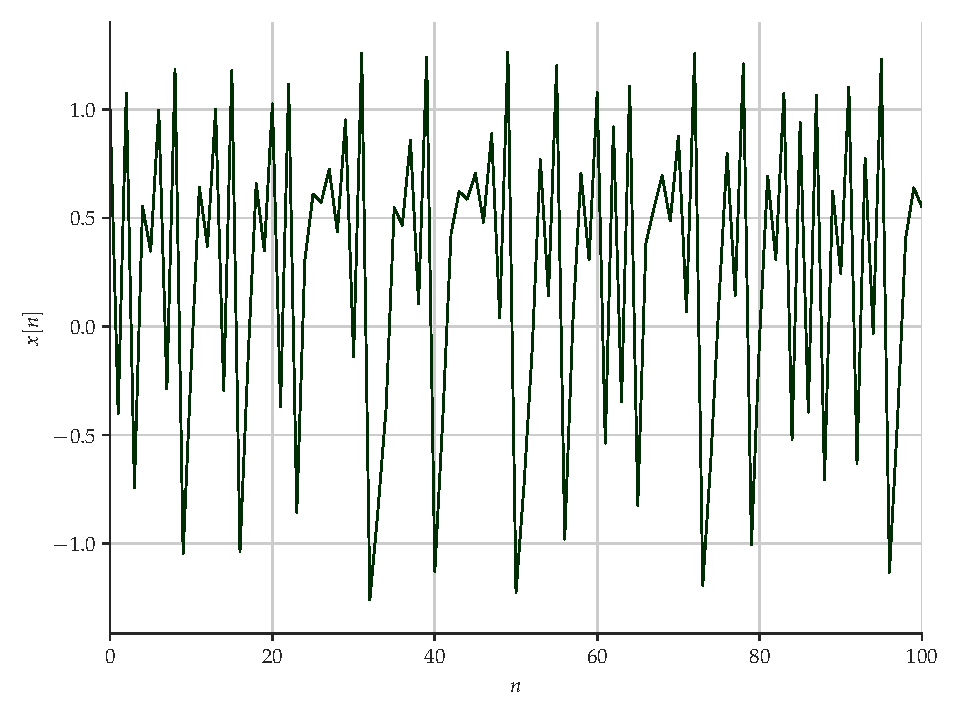
\includegraphics[scale=0.2]{serie-henon-x.pdf}
         %\caption{$y=5/x$}
     \end{subfigure}
     \centering
     \begin{subfigure}[t]{0.2\textwidth}
         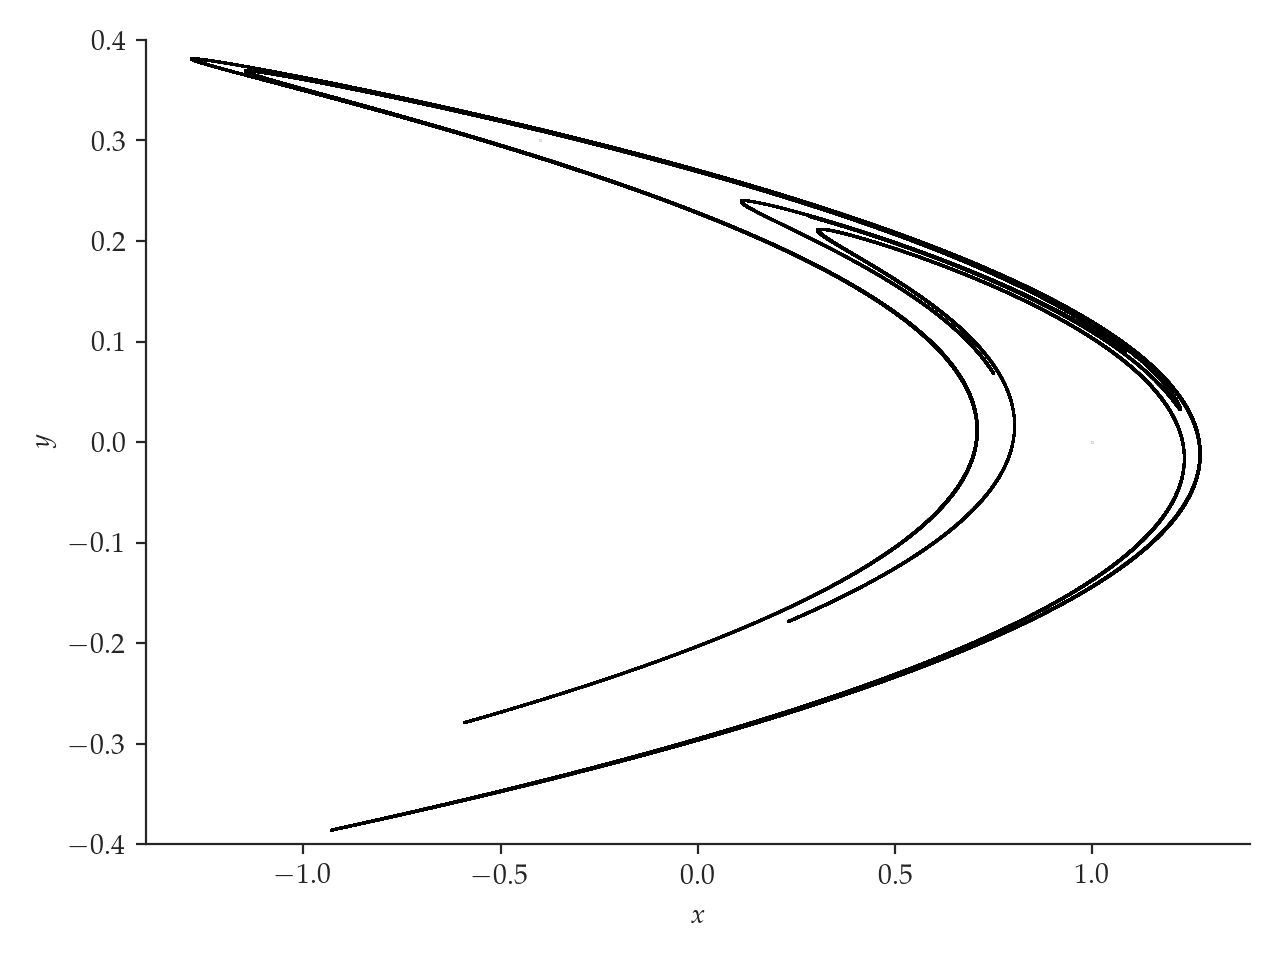
\includegraphics[scale=0.2]{mapa-de-henon.png}
         %\caption{$y=x$}
     \end{subfigure}
     \caption{À esquerda, as cem primeiras iterações da série temporal em $x$ do mapa de Hénon e, à direita, o atrator correspondente à simulação}
     \label{fig:henon}
\end{figure}

\subsubsection{Mapa logístico}

Conforme foi dito anteriormente, o outro sistema caótico a tempo discreto simulado foi o mapa logístico. Descrito em 1976 por Robert May, o mapa logístico representa uma das formas de modelar a população de uma determinada espécie em certos instantes de tempo \cite{may1976simple}. A equação a diferenças que descreve esse sistema pode ser vista abaixo:
\begin{equation}\label{eq:logistic}
x[n+1] = r\cdot x[n] \cdot (1 - x[n])
\end{equation}

Nesse caso, o sistema não chega a operar em caos para qualquer valor de $r$. Assim, como o estudo visa analisar o desempenho para sistemas caóticos, foi utilizado $r=3.86$, que, conforme será visto no diagrama de bifurcação abaixo, faz com que a série temporal dada pela equação (\ref{eq:logistic}) opere em caos. Novamente, foram simuladas $5000$ iterações, partindo de $x[0] = 0.5$, e a série gerada pode ser vista na figura \ref{fig:logistic}.
\begin{figure}[H]
     \begin{subfigure}[t]{0.2\textwidth} 
         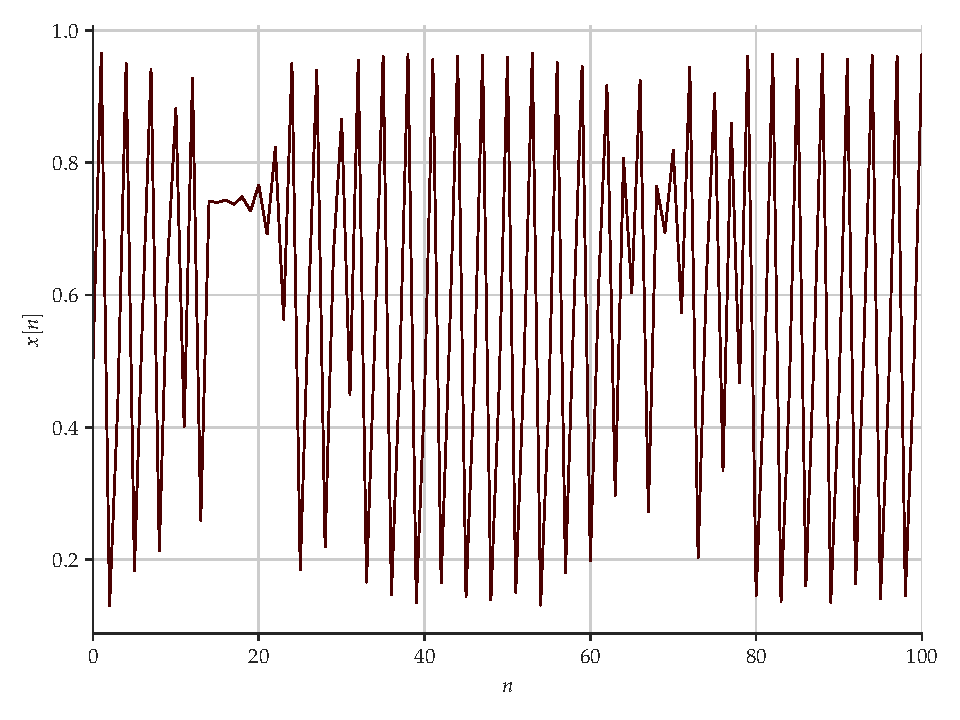
\includegraphics[scale=0.2]{serie-logistico.pdf}
         %\caption{$y=5/x$}
     \end{subfigure}
     \centering
     \begin{subfigure}[t]{0.2\textwidth} 
         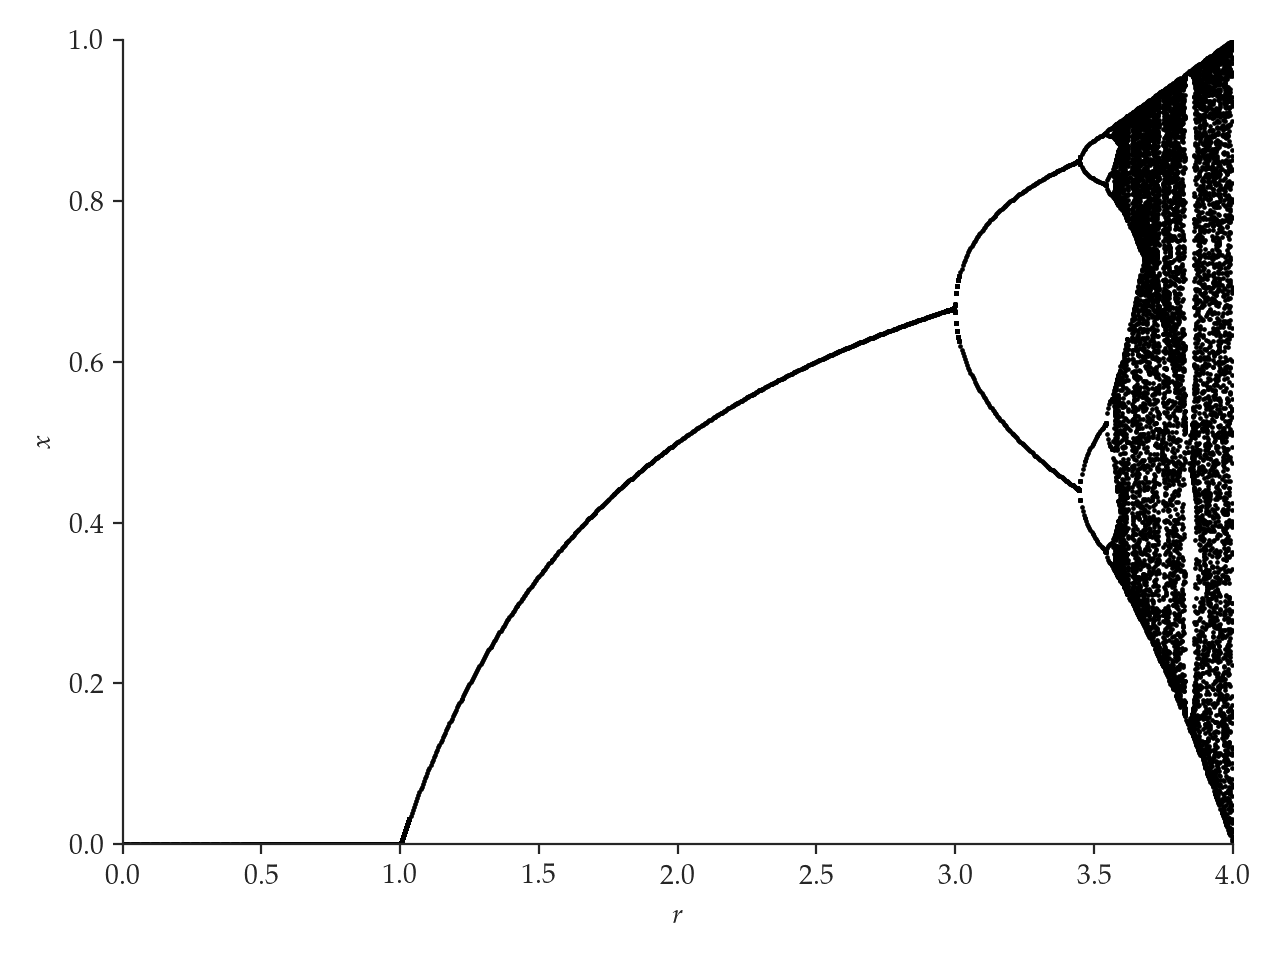
\includegraphics[scale=0.2]{mapa-logistico.png}
         %\caption{$y=x$}
     \end{subfigure}
     \caption{À esquerda, as cem primeiras iterações da série temporal do mapa logístico e, à direita, o diagrama de bifurcação deste sistema}
     \label{fig:logistic}
\end{figure}

\subsubsection{Sistema de Lorenz}

O sistema de Lorenz foi um dos sistemas dinâmicos caóticos a tempo contínuo abordados nessa pesquisa. Este sistema foi um dos primeiros grandes trabalhos envolvendo a noção de regime caótico, sendo considerado por muitos a pesquisa que inaugurou a área \cite{gleick1998chaos}. Lorenz modela, através de três equações diferenciais, o fluxo de um fluido em um volume uniformemente aquecido na camada inferior e uniformemente resfriado na camada superior \cite{lorenz1963deterministic}:
\begin{subequations}
\begin{equation}
\frac{dx}{dt} = -\sigma \cdot (x - y)
\end{equation}
\begin{equation}
\frac{dy}{dt} = x \cdot (\rho - z) - y
\end{equation}
\begin{equation}
\frac{dz}{dt} = x \cdot y - \beta \cdot z
\end{equation}
\end{subequations}

Para a simulação numérica foi considerado que $\sigma = 10$, $\beta = \frac{8}{3}$, $\rho = 28$ e foi utilizado $dt = 0.01$, gerando $5000$ amostras, assim como nos casos discretos. A figura \ref{fig:lorenz} mostra a série temporal na variável $x$ e o atrator de Lorenz para a condição inicial $[x(0)\; y(0)\; z(0)]^T = [0.1\; 0\; 0]^T$.
\begin{figure}[H]
     \begin{subfigure}[t]{0.2\textwidth} 
         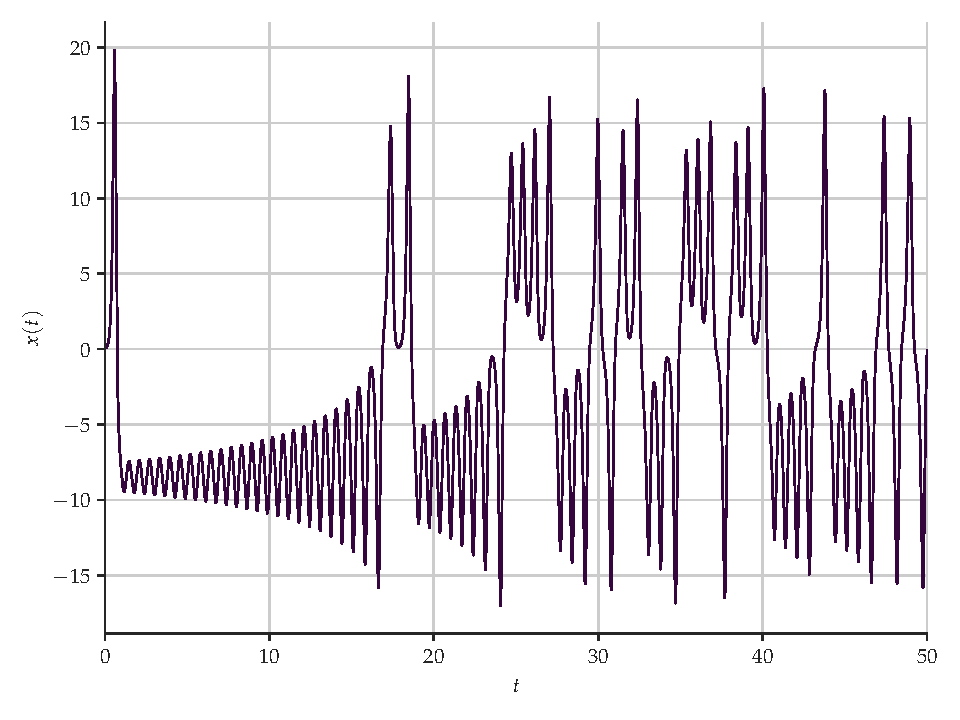
\includegraphics[scale=0.2]{serie-lorenz-x.pdf}
         %\caption{$y=5/x$}
     \end{subfigure}
     \centering
     \begin{subfigure}[t]{0.2\textwidth}
         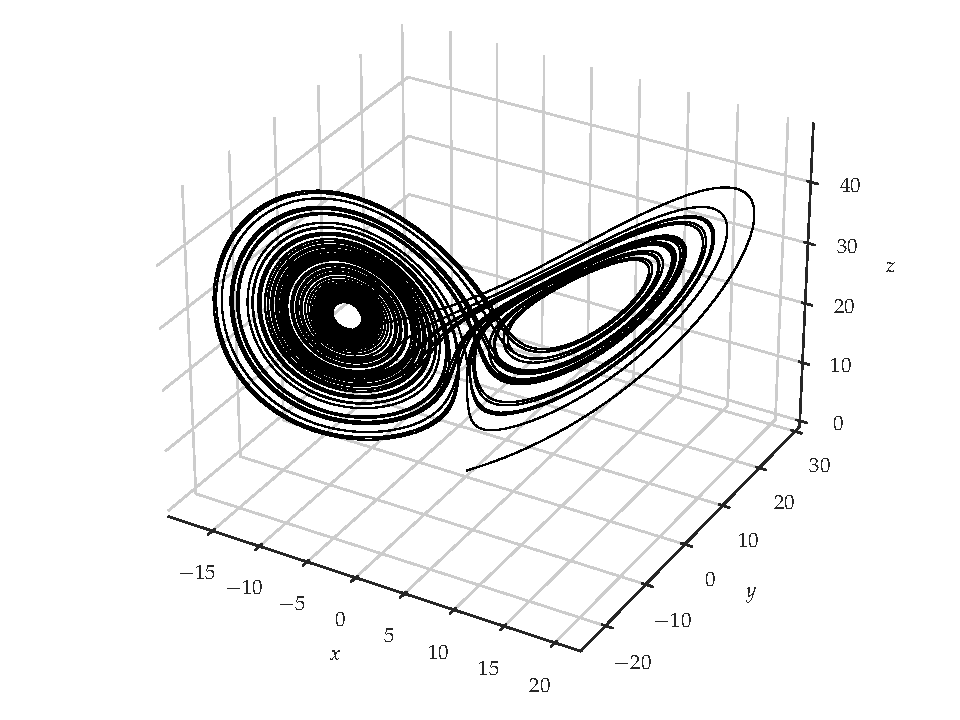
\includegraphics[scale=0.2]{diagrama-de-fases-lorenz.pdf}
         %\caption{$y=x$}
     \end{subfigure}
     \caption{À esquerda, a série temporal em $x$ do sistema de Lorenz simulado e, à direita, o diagrama de fases correspondente à simulação}
     \label{fig:lorenz}
\end{figure}

\subsubsection{Equações de Mackey-Glass}

Por fim, o último sistema caótico simulado, também contínuo, está associado às equações de Mackey-Glass, as quais modelam o controle hormonal da produção de células brancas do sangue e podem ser vistas abaixo \cite{mackey1977oscillation}:
\begin{subequations}
\begin{equation}
\frac{dP(t)}{dt} = \frac{\beta_0\cdot \theta^n}{\theta^n + P(t - \tau)^n} - \gamma\cdot P(t)
\end{equation}
\begin{equation}\label{eq:mackey-glass-chaos}
\frac{dP(t)}{dt} = \frac{\beta_0\cdot \theta^n \cdot P(t - \tau)}{\theta^n + P(t - \tau)^n} - \gamma\cdot P(t)
\end{equation}
\end{subequations}

Neste caso, a equação (\ref{eq:mackey-glass-chaos}) exibe comportamento caótico para valores mais altos de $\tau$. Para a simulação numérica, foi utilizado $n = 10$, $\gamma = 0.1$, $\beta = 0.2$, $\theta = 1$, $\tau = 22$, $dt = 1.0$ e $P(0^-)=0.1$, gerando novamente $5000$ amostras. A série e o atrator obtidos podem ser vistos na figura \ref{fig:mackey-glass}.
\begin{figure}[H]
     \begin{subfigure}[t]{0.2\textwidth}
         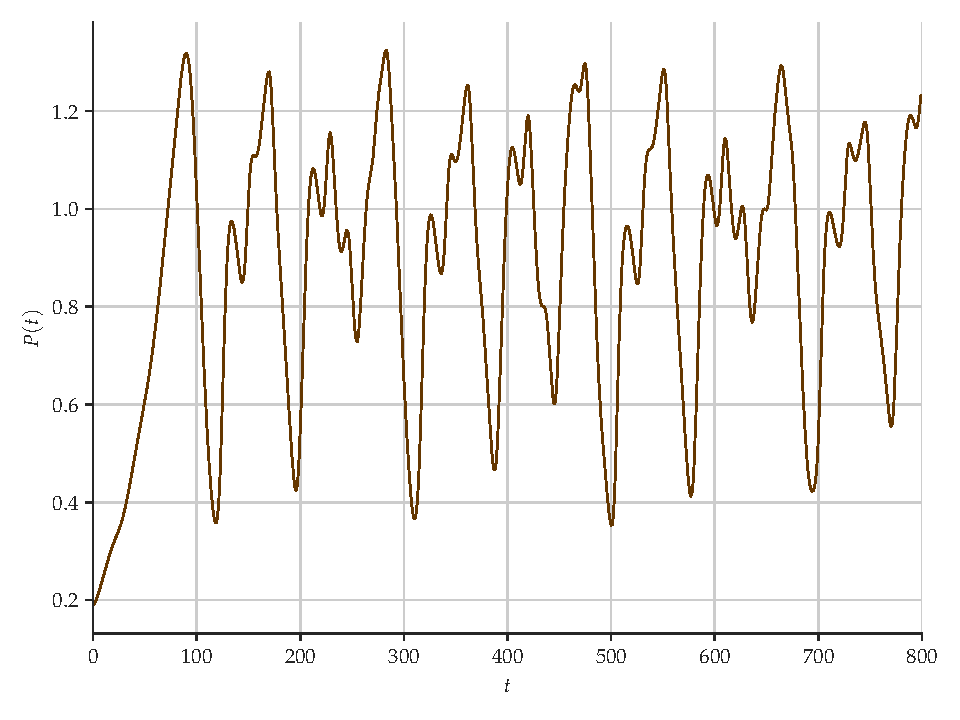
\includegraphics[scale=0.2]{serie-mackeyglass.pdf}
         %\caption{$y=5/x$}
     \end{subfigure}
     \centering
     \begin{subfigure}[t]{0.2\textwidth}
         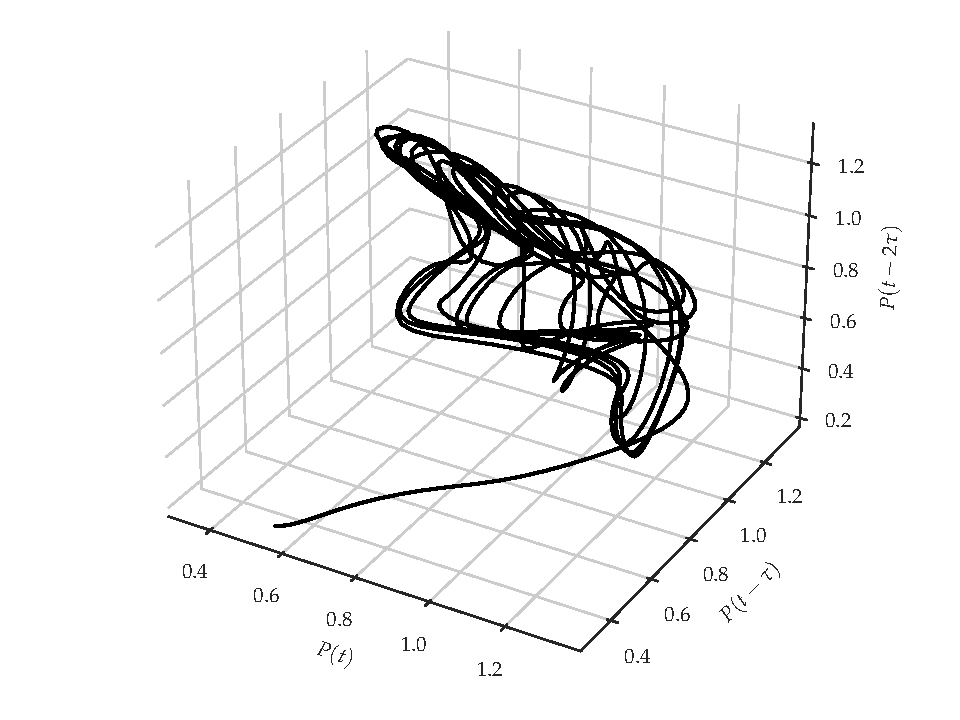
\includegraphics[scale=0.2]{atrator-mackeyglass.pdf}
         %\caption{$y=x$}
     \end{subfigure}
     \caption{À esquerda, a série temporal da equação (\ref{eq:mackey-glass-chaos}) exibida de $t = 0 $ a $t = 800$ e, à direita, o atrator correspondente à simulação}
     \label{fig:mackey-glass}
\end{figure}

\subsection{Redes neurais para previsão e configurações }

\BeforeBeginEnvironment{tabular}{\tiny}

Como foi mencionado na seção introdutória, através de uma busca em grade foram determinados os melhores valores dos hiperparâmetros das redes neurais estudadas. Para cada arquitetura, um conjunto de valores candidatos foi gerado para cada hiperparâmetro e todas as combinações possíveis foram avaliadas tendo em vista o desempenho do modelo em dados de validação. Nas próximas seções, apresentamos brevemente as redes neurais exploradas no trabalho bem como os detalhes da busca dos hiperparâmetros.

\subsubsection{MLP}

As redes MLP, como o nome já diz, são compostas por múltiplas camadas de neurônios artificiais do tipo \textit{perceptron}  \cite{rosenblatt1958perceptron}. Cada neurônio recebe os atributos $x_i, i = 1, \ldots, m$ de entrada e os pondera por pesos $w_i$. Em seguida, é aplicada uma função de ativação $\varphi(\cdot)$ sobre esta soma ponderada, acrescida de um termo de \textit{bias}, conforme indica a equação (\ref{eq:mlp-out}).
\begin{equation}\label{eq:mlp-out}
y = \varphi  \left(\sum_{i=1}^{m}w_i x_i + w_0 \right) = \varphi \left(\sum_{i=0}^{m}w_i x_i \right) = \varphi \left(\mathbf{w}^T \cdot \mathbf{x} \right)
\end{equation}

Tipicamente, uma rede neural MLP é composta por um número arbitrário $N_L$ de  camadas com $n$ neurônios do tipo \textit{perceptron}, com a característica de que as saídas dos neurônios da $l$-ésima camada são propagadas para a frente, servindo como as entradas de todos os neurônios da camada seguinte ($l+1$). Por isso, este tipo de rede é conhecida como totalmente conectada (ou densa) e pertence à categoria de modelos \textit{feedforward}. A figura \ref{fig:mlp-architecture} apresenta a estrutura típica das redes MLP.
\begin{figure}[H]
\centering
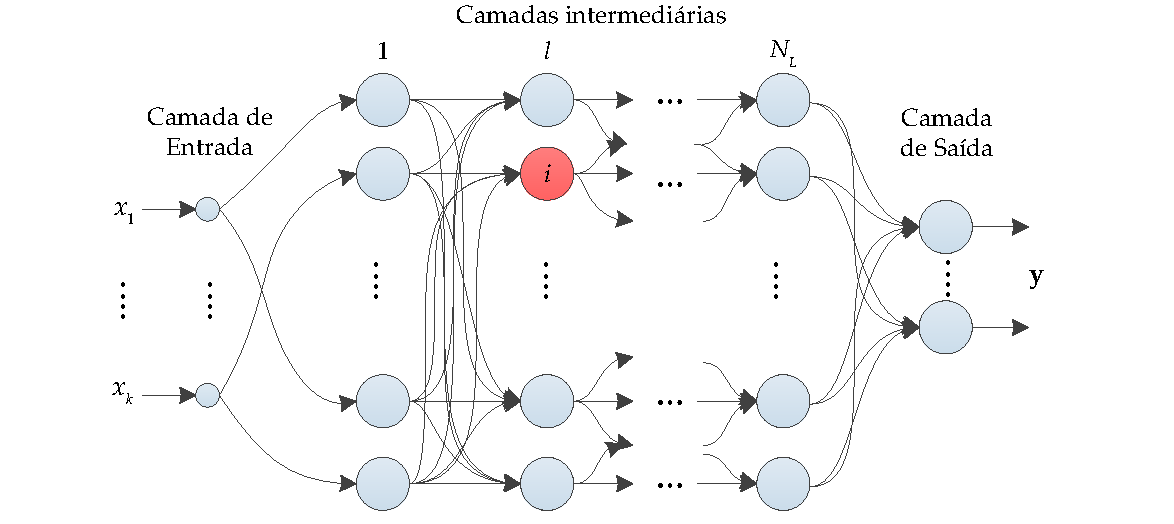
\includegraphics[scale = 0.3]{mlp-network.pdf}
\caption{Estrutura típica de uma rede MLP (figura adaptada de \cite{boccato2013novas}) }
\label{fig:mlp-architecture}
\end{figure}

O processo de treinamento de uma rede neural artificial normalmente é realizado com sequências de vetores de entrada $\mathbf{x}$, chamadas de \textit{mini-batch}, sendo que um período de treinamento é chamado de época \cite{geron2019hands}. Os pesos sinápticos $\textbf{w}$ são ajustados com um processo iterativo de forma a minimizar uma função custo $J(\textbf{w})$ que representa uma medida do erro entre as saídas geradas pela rede e as saídas desejadas. Para isso, é frequente o uso de algoritmos de otimização baseados em derivadas da função custo. Para esta pesquisa, foi utilizado o algoritmo Nadam \cite{dozat2016incorporating}. O processo de retropropagação do erro é empregado para viabilizar o cálculo das derivadas com relação aos pesos sinápticos dos neurônios situados nas camadas internas da rede.

Durante a etapa de validação, avaliamos diferentes tamanhos de \textit{batch}, se haveria ou não uma camada de \textit{batch normalization} na entrada da rede MLP, diferentes opções de função de ativação dos neurônios na camada intermediária, esquemas alternativos para a inicialização dos pesos, diferentes quantidades de neurônios na camada intermediária e, também, diferentes valores para a taxa de aprendizagem. 

A busca em grade considerou uma validação cruzada com $4$ \textit{folds} nos dados de treinamento, que correspondiam aos primeiros $4250$ valores. Essa proporção entre os dados de treinamento e de teste foi utilizada para todas as redes analisadas.

Vale reforçar que foi utilizada apenas uma camada intermediária em cada cenário. As melhores configurações obtidas podem ser vistas na tabela \ref{tab:mlp}.
\begin{table}[H]
\begin{center}
\begin{tabular}{c c c c c c c}
  \textbf{Cenário}  & \pbox{0.85cm}{\centering \textbf{\; \, \textit{Batch\newline normalization}}} & \pbox{0.4cm}{\centering \textbf{\textit{Batch size}}} & \pbox{0.65cm}{\centering \textbf{Função de ativação}} & \pbox{0.9cm}{\centering \textbf{Inicialização}} & \pbox{0.745cm}{\centering \textbf{Nº de neurônios}} & \pbox{1cm}{\centering \textbf{\, Taxa de\newline aprendizagem}}\\
 \hline
 \addlinespace
 \pbox{0.7cm}{\centering \textbf{Mapa de\newline Hénon}} & Não & $8$ & $\sigmoid$ & $\glorot\, \normal$ & $50$ & $0.003$\\  
  \addlinespace
 \pbox{0.7cm}{\centering \textbf{Mapa\newline logístico}} & Não & $2$ & $\tanh$ & $\glorot\, \uniform$ & $10$ & $0.003$\\ 
  \addlinespace
 \pbox{0.9cm}{\centering \textbf{Sistema de\newline Lorenz}} & Não & $2$ & $\selu$ & $\lecun\, \normal$ & $50$ & $0.001$\\ 
  \addlinespace
 \pbox{0.929cm}{\centering \textbf{Equações de\newline Mackey-Glass}} & Não & $4$ & $\tanh$ & $\glorot\, \normal$ & $5$ & $0.001$\\ 
\end{tabular}
\caption{Melhores parâmetros para a rede MLP nos cenários em análise}
\label{tab:mlp}
\end{center}
\end{table}

\subsubsection{LSTM e GRU}

Diferentemente das redes MLP, as redes recorrentes têm estruturas computacionais que podem armazenar os estados anteriores dos neurônios, possuindo também portas não-lineares que regulam o fluxo de informação de entrada e de saída da célula computacional \cite{haykin2010neural}. 

A diferença entre uma célula LSTM e uma célula GRU é a presença de um vetor de longo prazo $\mathbf{c}$ e um vetor de curto prazo $\mathbf{h}$ na LSTM, conforme indicado na figura \ref{fig:lstm}. 
\noindent{
\begin{figure}[H]
\begin{minipage}{0.2\textwidth}
\begin{center}
\scalebox{0.55}{
\begin{tikzpicture}[
    % GLOBAL CFG
    font=\sf \scriptsize,
    >=LaTeX,
    % Styles
    cell/.style={% For the main box
        rectangle, 
        rounded corners=5mm, 
        draw,
        very thick,
        },
    operator/.style={%For operators like +  and  x
        circle,
        draw,
        inner sep=-0.5pt,
        minimum height =.2cm,
        },
    function/.style={%For functions
        ellipse,
        draw,
        inner sep=1pt
        },
    ct/.style={% For external inputs and outputs
        circle,
        draw,
        line width = .75pt,
        minimum width=1cm,
        inner sep=1pt,
        },
    gt/.style={% For internal inputs
        rectangle,
        draw,
        minimum width=4mm,
        minimum height=3mm,
        inner sep=1pt
        },
    mylabel/.style={% something new that I have learned
        font=\scriptsize\sffamily
        },
    ArrowC1/.style={% Arrows with rounded corners
        rounded corners=.25cm,
        thick,
        },
    ArrowC2/.style={% Arrows with big rounded corners
        rounded corners=.5cm,
        thick,
        }
    ]

%Start drawing the thing...    
    % Draw the cell: 
    \node [cell, minimum height =4cm, minimum width=6cm] at (0,0){} ;

    % Draw inputs named ibox#
    \node [gt] (ibox1) at (-2,-0.75) {$\sigma$};
    \node [gt] (ibox2) at (-1.5,-0.75) {$\sigma$};
    \node [gt, minimum width=1cm] (ibox3) at (-0.5,-0.75) {$\tanh$};
    \node [gt] (ibox4) at (0.5,-0.75) {$\sigma$};

   % Draw opérators   named mux# , add# and func#
    \node [operator] (mux1) at (-2,1.5) {$\times$};
    \node [operator] (add1) at (-0.5,1.5) {+};
    \node [operator] (mux2) at (-0.5,0) {$\times$};
    \node [operator] (mux3) at (1.5,0) {$\times$};
    \node [function] (func1) at (1.5,0.75) {$\tanh$};

    % Draw External inputs? named as basis c,h,x
    \node[] (c) at (-4,1.5) {$\mathbf{c}(t-1)$};
    \node[] (h) at (-4,-1.5) {$\mathbf{h}(t-1)$};
    \node[] (x) at (-2.5,-3) {$\mathbf{x}(t)$};

    % Draw External outputs? named as basis c2,h2,x2
    \node[] (c2) at (4,1.5) {$\mathbf{c}(t)$};
    \node[] (h2) at (4,-1.5) {$\mathbf{h}(t)$};
    \node[] (x2) at (2.5,3) {$\mathbf{y}(t)$};
    
    % Draw internals functions, named as basis fi,ii,ci,oi
    \node[] (fi) at (-2.35,-0.25) {$\mathbf{f}(t)$};
    \node[] (ii) at (-1.5,0.2) {$\mathbf{i}(t)$};
    \node[] (ci) at (-0.1,-0.35) {$\mathbf{\tilde{c}}(t)$};
	\node[] (oi) at (0.5,0.2) {$\mathbf{o}(t)$};       
    
% Start connecting all.
    %Intersections and displacements are used. 
    % Drawing arrows    
    \draw [ArrowC1] (c) -- (mux1) -- (add1) -- (c2);

    % Inputs
    \draw [ArrowC2] (h) -| (ibox4);
    \draw [ArrowC1] (h -| ibox1)++(-0.5,0) -| (ibox1); 
    \draw [ArrowC1] (h -| ibox2)++(-0.5,0) -| (ibox2);
    \draw [ArrowC1] (h -| ibox3)++(-0.5,0) -| (ibox3);
    \draw [ArrowC1] (x) -- (x |- h)-| (ibox3);

    % Internal
    \draw [->, ArrowC2] (ibox1) -- (mux1);
    \draw [->, ArrowC2] (ibox2) |- (mux2);
    \draw [->, ArrowC2] (ibox3) -- (mux2);
    \draw [->, ArrowC2] (ibox4) |- (mux3);
    \draw [->, ArrowC2] (mux2) -- (add1);
    \draw [->, ArrowC1] (add1 -| func1)++(-0.5,0) -| (func1);
    \draw [->, ArrowC2] (func1) -- (mux3);

    %Outputs
    \draw [->, ArrowC2] (mux3) |- (h2);
    \draw [->] (add1) |- (c2);
    \draw (c2 -| x2) ++(0,-0.1) coordinate (i1);
    \draw [-, ArrowC2] (h2 -| x2)++(-0.5,0) -| (i1);
    \draw [->, ArrowC2] (i1)++(0,0.2) -- (x2);

\end{tikzpicture}}
\end{center}
\end{minipage}
\; \; \; \; \; \; \; \;
\begin{minipage}{0.2\textwidth}
\begin{center}
{\tiny
$$\mathbf{f}(t) = \sigma(\mathbf{W}_f [\mathbf{h}(t-1), \mathbf{x}(t)] + \mathbf{b}_f)$$
$$\mathbf{i}(t) = \sigma(\mathbf{W}_i [\mathbf{h}(t-1), \mathbf{x}(t)] + \mathbf{b}_i)$$
$$\mathbf{\tilde{c}}(t) = \tanh(\mathbf{W}_c [\mathbf{h}(t-1), \mathbf{x}(t)] + \mathbf{b}_c)$$
$$\mathbf{c}(t) = \mathbf{f}(t) \otimes \mathbf{c}(t-1) + \mathbf{i}(t) \otimes \mathbf{\tilde{c}}(t)$$
$$\mathbf{o}(t) = \sigma(\mathbf{W}_o [\mathbf{h}(t-1), \mathbf{x}(t)] + \mathbf{b}_o)$$
$$\mathbf{y}(t) = \mathbf{h}(t) = \mathbf{o}(t) \otimes \tanh (\mathbf{c}(t))$$}
\end{center}
\end{minipage}
\caption{Estrutura e equações de uma célula LSTM}
\label{fig:lstm}
\end{figure}
}

As LSTMs manipulam o vetor $\mathbf{c}(t)$, aprendendo durante o treinamento o que deve ser guardado nele, o que deve ser descartado e o que deve ser aproveitado para gerar a saída $\mathbf{h}(t)$. Dessa forma, podemos dizer que a atualização do vetor de estados $\mathbf{c}(t)$ é feita com o descarte de informações e a incorporação de novidades vindas da entrada. 

A célula GRU é uma versão simplificada da célula LSTM e funciona de uma forma bem similar. Nela há somente o vetor de estados de curto prazo  $\mathbf{h}$, assim, para que uma memória seja mantida, o conteúdo do local em questão deve ser primeiramente apagado.

À semelhança das redes MLP, o treinamento das redes LSTM e GRU também é realizado através de algoritmos de otimização baseados em derivadas da função custo; a diferença é que agora é necessário propagar as derivadas ao longo da estrutura e, também, ao longo do tempo devido às realimentações. O algoritmo BPTT (\textit{backpropagation-through-time}) representa a extensão do \textit{backpropagation} para o cenário das redes recorrentes \cite{geron2019hands}. 

Para a busca em grade, foi considerado um esquema de validação do tipo \textit{holdout}. Esse processo dividiu o conjunto de treinamento (novamente composto por $85\%$ dos dados gerados) em $4$ seções. Cada seção era composta por uma fração dos dados de treinamento, sendo que cada seção incluía a seção anterior no seu conjunto de dados.

Por exemplo, a segunda seção obtida pelo \textit{holdout} inclui a primeira seção e mais algumas amostras, além de uma subdivisão de validação que será utilizada para avaliar o resultado. Com isso, obtém-se conjuntos sequenciais de dados para avaliação do desempenho. Esse procedimento é necessário para as redes recorrentes, pois a relação temporal entre os dados de entrada deve ser levada em conta.

Foi avaliado o tamanho do \textit{batch}, a inicialização dos pesos, o número de neurônios recorrentes na camada intermediária, e a taxa de aprendizagem, novamente utilizando apenas uma camada intermediária e mantendo a função de ativação usual da célula recorrente ($\tanh$). Por conta disso, para o sistema de Lorenz, foi feito um ajuste de escala para evitar a saturação dos neurônios.

Os resultados obtidos para a LSTM e para a GRU podem ser vistos nas tabelas \ref{tab:lstm} e \ref{tab:gru}, respectivamente.
\begin{table}[H]
\begin{center}
\begin{tabular}{c c c c c}
  \textbf{Cenário} & \pbox{0.4cm}{\centering \textbf{\textit{Batch size}}} & \pbox{0.9cm}{\centering \textbf{Inicialização}} & \pbox{0.745cm}{\centering \textbf{Nº de neurônios}} & \pbox{1cm}{\centering \textbf{\, Taxa de\newline aprendizagem}}\\
 \hline
 \addlinespace
 \pbox{0.7cm}{\centering \textbf{Mapa de\newline Hénon}} & $4$ & $\glorot\, \normal$ & $15$ & $0.005$\\  
  \addlinespace
 \pbox{0.7cm}{\centering \textbf{Mapa\newline logístico}} & $2$ & $\glorot\, \uniform$ & $100$ & $0.008$\\ 
  \addlinespace
 \pbox{0.9cm}{\centering \textbf{Sistema de\newline Lorenz}} & $4$ & $\glorot\, \uniform$ & $15$ & $0.003$\\ 
  \addlinespace
 \pbox{0.929cm}{\centering \textbf{Equações de\newline Mackey-Glass}} & $2$ & $\glorot\, \uniform$ & $50$ & $0.003$\\ 
\end{tabular}
\caption{Melhores parâmetros para a rede LSTM nos cenários em análise}
\label{tab:lstm}
\end{center}
\end{table}
\begin{table}[H]
\begin{center}
\begin{tabular}{c c c c c}
  \textbf{Cenário} & \pbox{0.4cm}{\centering \textbf{\textit{Batch size}}} & \pbox{0.9cm}{\centering \textbf{Inicialização}} & \pbox{0.745cm}{\centering \textbf{Nº de neurônios}} & \pbox{1cm}{\centering \textbf{\, Taxa de\newline aprendizagem}}\\
 \hline
 \addlinespace
 \pbox{0.7cm}{\centering \textbf{Mapa de\newline Hénon}} & $4$ & $\glorot\, \normal$ & $30$ & $0.003$\\  
  \addlinespace
 \pbox{0.7cm}{\centering \textbf{Mapa\newline logístico}} & $2$ & $\glorot\, \normal$ & $100$ & $0.003$\\ 
  \addlinespace
 \pbox{0.9cm}{\centering \textbf{Sistema de\newline Lorenz}} & $8$ & $\glorot\, \uniform$ & $30$ & $0.001$\\ 
  \addlinespace
 \pbox{0.929cm}{\centering \textbf{Equações de\newline Mackey-Glass}} & $2$ & $\glorot\, \uniform$ & $10$ & $0.005$\\ 
\end{tabular}
\caption{Melhores parâmetros para a rede GRU nos cenários em análise}
\label{tab:gru}
\end{center}
\end{table}

\subsubsection{ESN}

O último modelo de previsão considerado no trabalho foi a rede neural com estados de eco, a qual também é uma rede recorrente, assim como a LSTM, mas apresenta um modo de operação e um esquema de treinamento bem diferentes. 

As equações abaixo descrevem a ESN, sendo $\mathbf{x}(n)$ o vetor de entrada, $\mathbf{W}_{in} \in \mathbb{R}^{N \times K}$ os pesos da camada de entrada, $\mathbf{u}(t)$ o vetor que representa as ativações dos $N$ neurônios não-lineares totalmente conectados do reservatório, representando os estados da rede, $\mathbf{W} \in \mathbb{R}^{N \times N}$ os pesos das conexões recorrentes do reservatório, $\mathbf{f}(\cdot)$ denota as funções de ativação das unidades internas da rede, $\mathbf{W}_{out} \in \mathbb{R}^{L \times N}$ é a matriz dos pesos da camada de saída e, por fim, $\mathbf{y}(n)$ denota as saídas da rede.
\begin{subequations}
\begin{equation}
\mathbf{u}(n+1) = \mathbf{f}(\mathbf{W}_{in} \cdot \mathbf{x}(n+1) + \mathbf{W} \cdot \mathbf{u}(n))
\end{equation}
\begin{equation}
\mathbf{y}(n+1) = \mathbf{W}_{out} \cdot \mathbf{u}(n+1)
\end{equation}
\end{subequations}

O grande diferencial prático desta rede é que os pesos das conexões recorrentes dentro do reservatório $\mathbf{W}$ são ajustados com valores fixos antes do treinamento da camada de saída. Esses parâmetros são determinados tendo em vista a propriedade de estados de eco, existindo alguns métodos simples para a criação aleatória dos pesos e que asseguram a propriedade, conforme demonstrado em \cite{jaeger2007echo}. 

Devido a isso, o ajuste dos neurônios na camada de saída pode ser realizado com um procedimento de regressão linear, sem necessitar de um treinamento iterativo, como nas outras redes recorrentes. Esse fato economiza tempo de processamento e garante que será atingido o mínimo global da função custo utilizada.

Para esta rede foi realizada uma busca em grade para determinar o número de neurônios no reservatório e o valor para o raio espectral, que determina o maior valor singular da matriz de pesos do reservatório. Por tratar-se de uma rede recorrente, também foi utilizado o processo de \textit{holdout} descrito na seção anterior. Vale também mencionar que a taxa de vazamento, que representa a velocidade com a qual o reservatório atualiza suas dinâmicas, foi fixada em $0.9$ para todos os cenários.

A tabela \ref{tab:esn} exibe as melhores configurações para a ESN em cada um dos cenários.
\begin{table}[H]
\begin{center}
\begin{tabular}{c c c c c}
  \textbf{Parâmetro} & \pbox{0.7cm}{\centering \textbf{Mapa de\newline Hénon}} & \pbox{0.6cm}{\centering \textbf{Mapa\newline logístico}} & \pbox{1.0cm}{\centering \textbf{Sistema de\newline Lorenz}} & \pbox{1.1cm}{\centering \textbf{Equações de\newline Mackey-Glass}}\\
 \hline
 \addlinespace
 {\centering \textbf{Raio espectral}} & $0.1$ & $0.1$ & $0.2$ & $0.4$\\  
  \addlinespace
 {\centering \textbf{Nº de neurônios}} & $500$ & $500$ & $120$ & $500$\\ 
\end{tabular}
\caption{Melhores parâmetros para a rede ESN nos cenários em análise}
\label{tab:esn}
\end{center}
\end{table}

\subsection{Análise do melhor valor para $K$}

Com as melhores configurações para cada rede e cenário obtidas, foi analisada a progressão do erro quadrático médio para cada valor de $K$. A faixa de valores para $K$ a ser testada foi determinada utilizando a autocorrelação parcial das séries temporais de cada sistema analisado, levando em consideração os valores de $K$ que têm as autocorrelações parciais mais relevantes.

Para realizar esse procedimento, cada rede (com as configurações ótimas) foi treinada utilizando $85\%$ dos dados gerados, sendo que $10\%$ dos dados de treinamento foi utilizado como o conjunto de validação (nas redes MLP, LSTM e GRU). Em seguida, com o modelo treinado, foi avaliado o EQM no conjunto de teste (que corresponde às últimas 750 amostras). Esse processo foi realizado $5$ vezes para cada $K$, obtendo assim um valor médio e desvio-padrão para cada modelo e em cada cenário. 

Vale reforçar que, como o ajuste de parâmetros da ESN possui solução em forma fechada, não foi necessário utilizar um conjunto de validação no treinamento. No caso da MLP, LSTM e GRU, o processo iterativo de ajuste dos pesos utilizou um conjunto de validação de forma a seguir o procedimento de \textit{early stopping} para evitar o sobreajuste da rede.

A figura \ref{fig:mse-progression} mostra a progressão do EQM observada em cada cenário para cada uma das redes estudadas. 
\begin{figure}[H]
     \begin{subfigure}[t]{0.2\textwidth} 
         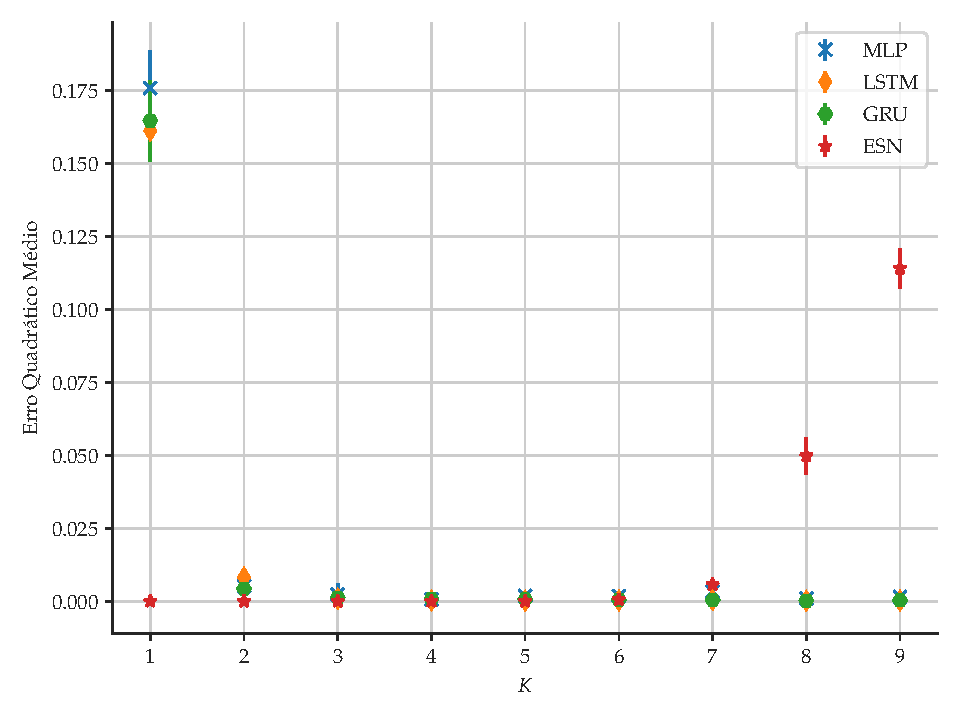
\includegraphics[scale=0.2]{progressao-k-henon.pdf}
         \caption{Mapa de Hénon}
     \end{subfigure}
     \centering
     \begin{subfigure}[t]{0.2\textwidth} 
         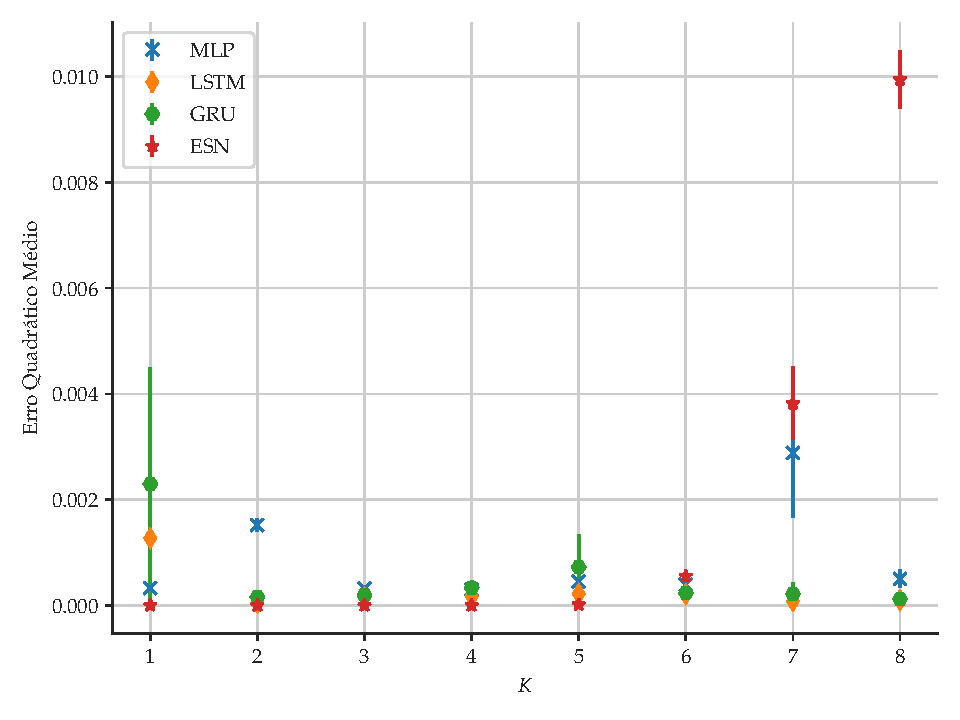
\includegraphics[scale=0.2]{progressao-k-logistic.pdf}
         \caption{Mapa logístico}
     \end{subfigure}
     \centering
     \begin{subfigure}[t]{0.2\textwidth}
         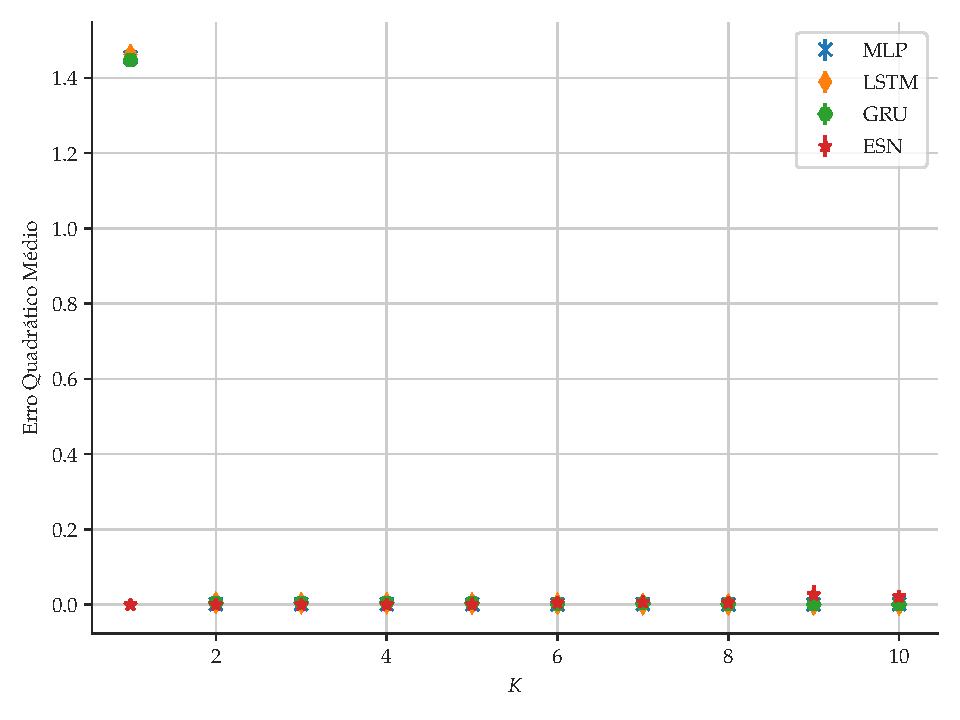
\includegraphics[scale=0.2]{progressao-k-lorenz.pdf}
         \caption{Sistema de Lorenz}
     \end{subfigure}
     \centering
     \begin{subfigure}[t]{0.2\textwidth} 
         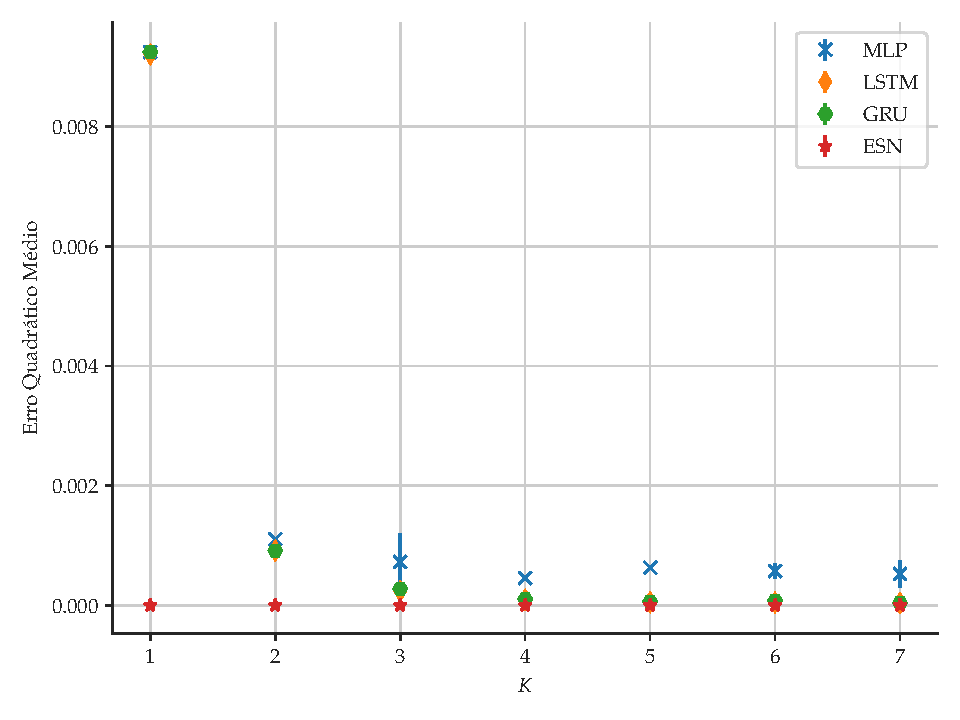
\includegraphics[scale=0.2]{progressao-k-mackeyglass.pdf}
         \caption{Equações de Mackey-Glass}
     \end{subfigure}  
     \centering   
     \caption{Progressão do erro quadrático médio para cada valor de $K$ nos cenários avaliados para todas as redes neurais testadas}
     \label{fig:mse-progression}
\end{figure}

\section{Resultados}

Após identificarmos o melhor valor de $K$ para cada modelo, realizou-se novamente o processo mencionado na seção anterior e foi obtido o EQM para as melhores configurações (parâmetros e $K$) para cada modelo, em todos os cenários. 

A figura \ref{fig:model-comparison} exibe o comparativo dos melhores desempenhos das redes neurais analisadas, e a figura \ref{fig:series-comparison} mostra uma comparação da predição em si de cada modelo nos cenários onde a diferença foi mais perceptível visualmente.
\begin{figure}[!h]
     \begin{subfigure}[t]{0.24\textwidth}
         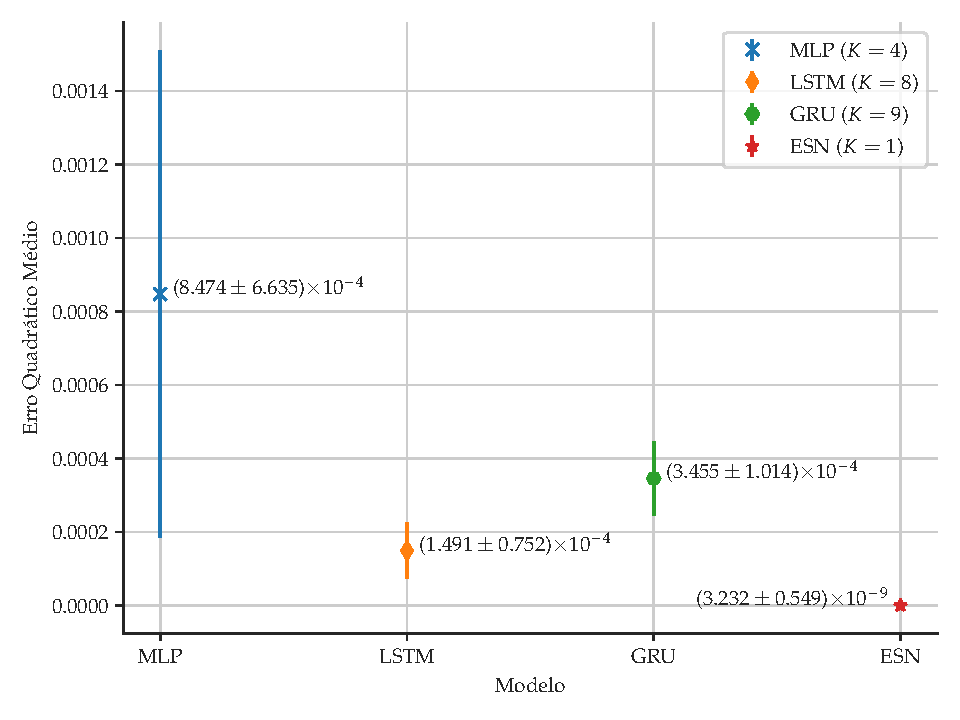
\includegraphics[scale=0.24]{comparacao-k-henon.pdf}
         \caption{Mapa de Hénon}
     \end{subfigure}
     \centering
     \begin{subfigure}[t]{0.24\textwidth} 
         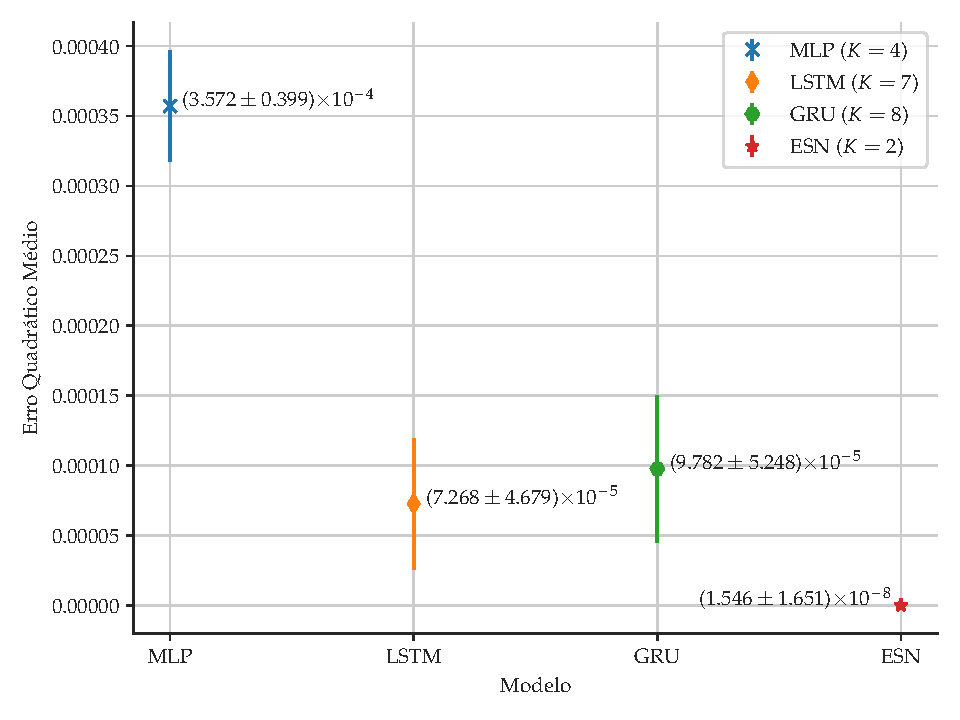
\includegraphics[scale=0.24]{comparacao-k-logistic.pdf}
         \caption{Mapa logístico}
     \end{subfigure}
     \centering
     \begin{subfigure}[t]{0.24\textwidth}
         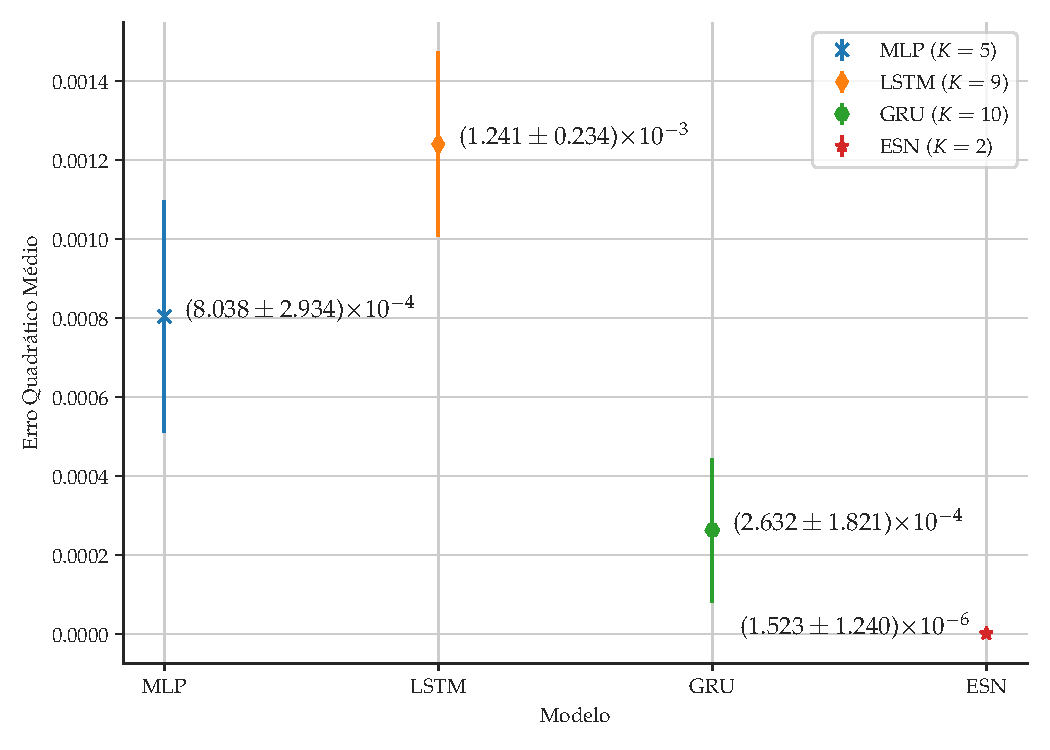
\includegraphics[scale=0.24]{comparacao-k-lorenz.pdf}
         \caption{Sistema de Lorenz}
     \end{subfigure}
     \centering
     \begin{subfigure}[t]{0.24\textwidth} 
         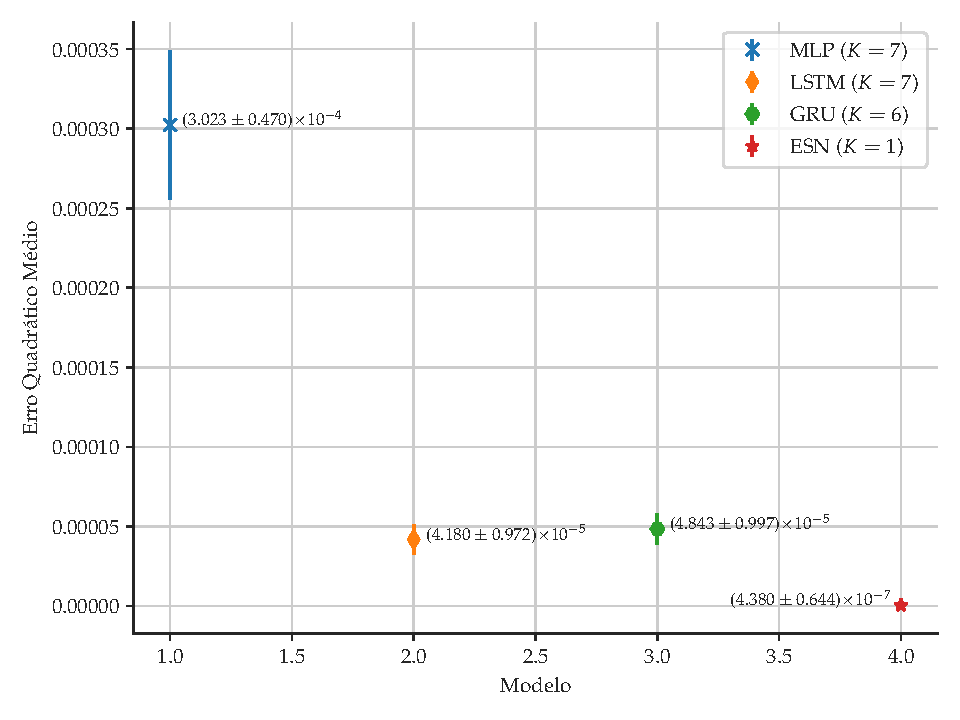
\includegraphics[scale=0.24]{comparacao-mackeyglass.pdf}
         \caption{Equações de Mackey-Glass}
     \end{subfigure}  
     \centering   
     \caption{Comparação do melhor desempenho obtido por cada modelo nos cenários testados}
     \label{fig:model-comparison}
\end{figure}
\begin{figure}[!ht]
     \begin{subfigure}[t]{0.2\textwidth} 
         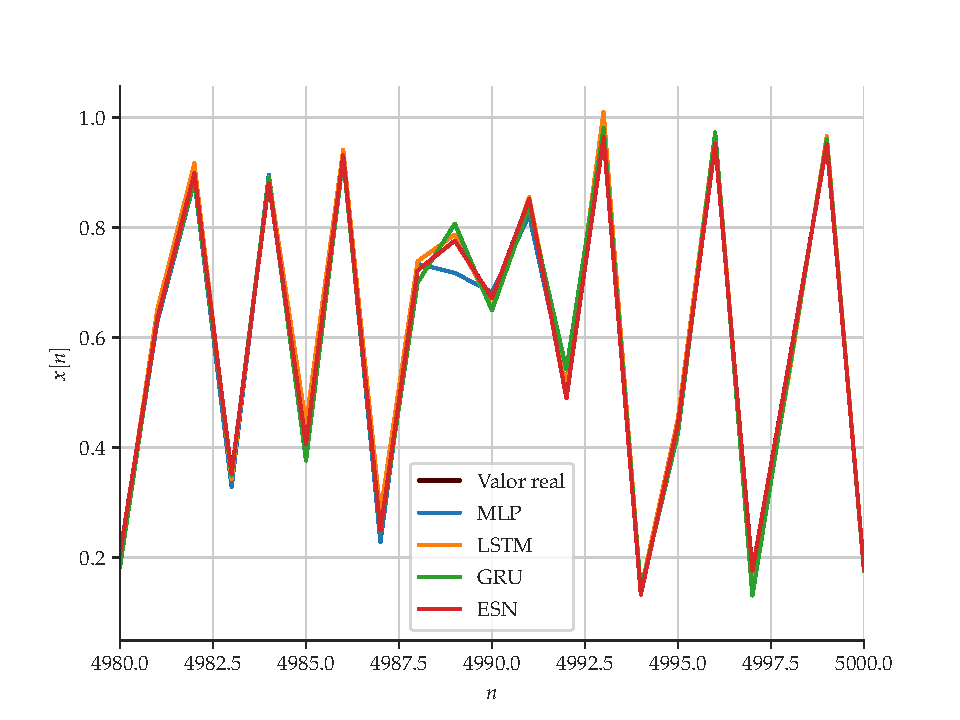
\includegraphics[scale=0.2]{vs-logistic-zoom.pdf}
         \caption{Mapa logístico}
     \end{subfigure}
     \centering
     \begin{subfigure}[t]{0.2\textwidth}
         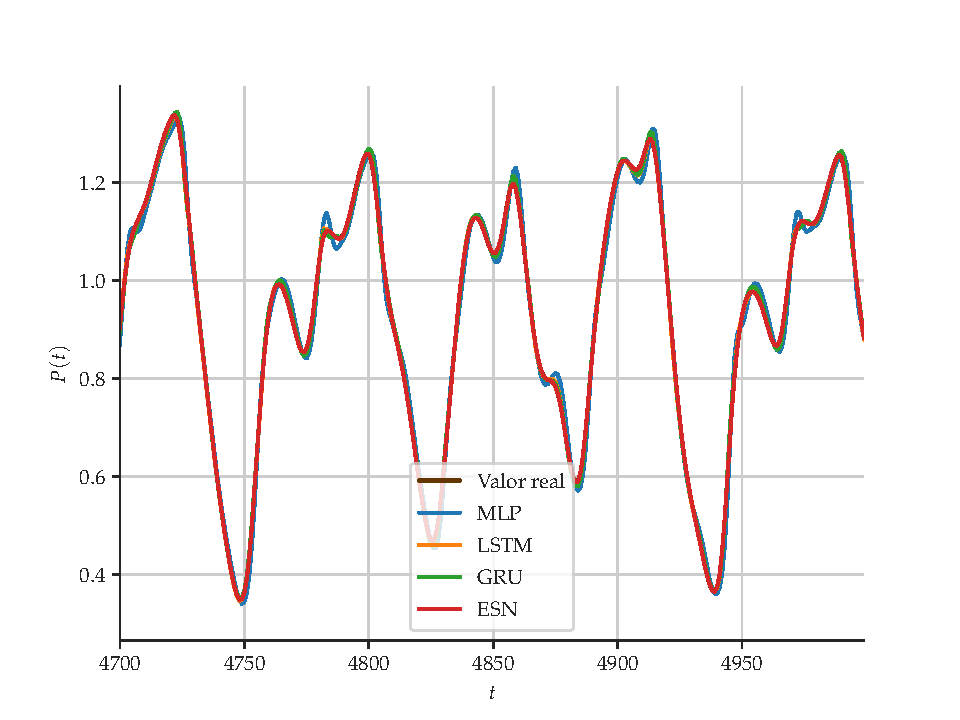
\includegraphics[scale=0.2]{vs-mackeyglass-zoom.pdf}
         \caption{Equações de Mackey-Glass}
     \end{subfigure}
     \centering     
     \caption{Comparação da predição realizada por cada modelo nos cenários do mapa logístico e das equações de Mackey-Glass}
     \label{fig:series-comparison}
\end{figure}

\section{Análise e Conclusão}

Analisando os resultados obtidos, percebe-se que, com exceção do cenário do sistema de Lorenz, a rede MLP foi consideravelmente pior do que as redes recorrentes. Também percebe-se que, dentre as redes recorrentes, a ESN obteve um EQM bem inferior ao obtido pela LSTM e pela GRU.

O desempenho inferior da rede MLP com relação às redes recorrentes provavelmente decorre do fato de que a relação temporal presente na LSTM, GRU e ESN auxilia na modelagem da dinâmica da série temporal. Já o pior desempenho da LSTM na série temporal do sistema de Lorenz provavelmente está relacionado aos efeitos estocásticos presentes no ajuste dos pesos sinápticos dessa rede neural que, conforme indicado em \cite{doya1992bifurcations}, é uma dificuldade em seu treinamento.

Algo interessante de mencionar é que, no geral, os desempenhos de todos os modelos estudados foram consideravelmente bons nas séries temporais dos sistemas a tempo contínuo (sistema de Lorenz e equações de Mackey-Glass), sendo que as diferenças foram mais pronunciadas na série temporal do mapa de Hénon e do mapa logístico. Provavelmente, a suavidade presente nas séries de Lorenz e de Mackey-Glass facilita a modelagem do preditor, além do fato de que as séries temporais mencionadas são bem menos erráticas se comparadas às séries de Hénon e do mapa logístico.

O principal resultado observado foi que o modelo preditor utilizando a rede com estados de eco obteve um desempenho bem superior aos outros modelos, em todos os cenários. O erro quadrático médio foi tão baixo que, observando a predição nos dados de teste, praticamente não há diferença entre os valores reais e os valores previstos. Essa superioridade da ESN também é realçada na imagem  comparativa do EQM, que indica que a ESN  atingiu patamares de erro cerca de $100$ ou até $10000$ vezes menores que os outros modelos. 

Esse resultado, aliado ao fato de que o treinamento da ESN é bem menos custoso computacionalmente se comparado ao das outras redes, mostra que esta rede é uma boa alternativa para futuros estudos de modelos preditores de séries temporais. Além disso, conforme mostrado em outros trabalhos como \cite{jaeger2004harnessing, jaeger2007echo, boccato2013novas}, a ESN também é uma boa ferramenta para outras tarefas de extração de informação, como em equalização de canais e separação de fontes. 

Como sugestão de trabalhos futuros, pode ser avaliada a eficácia da ESN em reconstruir atratores através de séries temporais experimentais de sistemas caóticos. Se o desempenho para essa tarefa for tão bom quanto o obtido na predição das séries estudadas, a ESN pode tornar-se uma ferramenta ainda mais poderosa para a modelagem de sistemas com dinâmica caótica.

\bibliographystyle{ieeetr}
{\scriptsize
\bibliography{bib}
}
\pdfinfo{
  /Title  (Congresso PIBIC 2021 - João P. Pagnan)
  /CreationDate (D:20040502195600)
}


\end{document}